\documentclass[10pt,letterpaper]{article}
\usepackage[left=0.75in,right=0.75in,top=0.68in,bottom=0.72in]{geometry}
\usepackage[hyphens]{url}
\usepackage[hidelinks]{hyperref}
\usepackage{graphicx}
\usepackage{newtxtext,newtxmath}
\usepackage[font=small,labelfont=bf]{caption}
\usepackage{array,booktabs,tabularx}
\urlstyle{rm}
\frenchspacing
\pagestyle{empty}

\pdfinfo{
/TemplateVersion (2027.1)
/Subject (Anonymous supplementary technical appendix)
}

\setcounter{secnumdepth}{0}
\renewcommand{\thefigure}{A\arabic{figure}}
\newcommand{\suppsection}[1]{\vspace{2pt}{\large\bfseries #1\par}\vspace{5pt}}

\begin{document}
\begin{center}
  {\LARGE\bfseries Supplementary Material for ContextLens\par}
  \vspace{3pt}
  {\large\bfseries Technical Architecture and Data Flow\par}
  \vspace{4pt}
  {\normalsize Anonymous Submission\par}
\end{center}
\vspace{6pt}

\noindent\textbf{Anonymous artifacts.}
An anonymous repository containing the complete source code and demonstration video is available at
\url{https://anonymous.4open.science/r/ContextLens-B7C0/README.md}.
\vspace{8pt}

\suppsection{Supplement A. Software Architecture}
\noindent
\begin{minipage}[t]{0.473\textwidth}
ContextLens separates interaction, evidence compilation, data services, and presentation (Figure~\ref{fig:architecture}). A local controller receives a dated address and maintains the investigation state. The evidence compiler resolves temporal place identity before retrieval. It then normalizes records, admits relations and claims, and projects the audited objects into a dossier.
\end{minipage}\hfill
\begin{minipage}[t]{0.473\textwidth}
The packaged snapshot and live adapters share a normalized record contract. Source Passports retain the evidence identifier, original URI, temporal scope, and normalization state. Model-assisted interpretation occurs after the claim audit. Returned identifiers are intersected with the admitted set before a summary is exposed. Model failure therefore affects the optional summary, not the underlying dossier.
\end{minipage}
\vspace{10pt}

\begin{center}
  \centering
  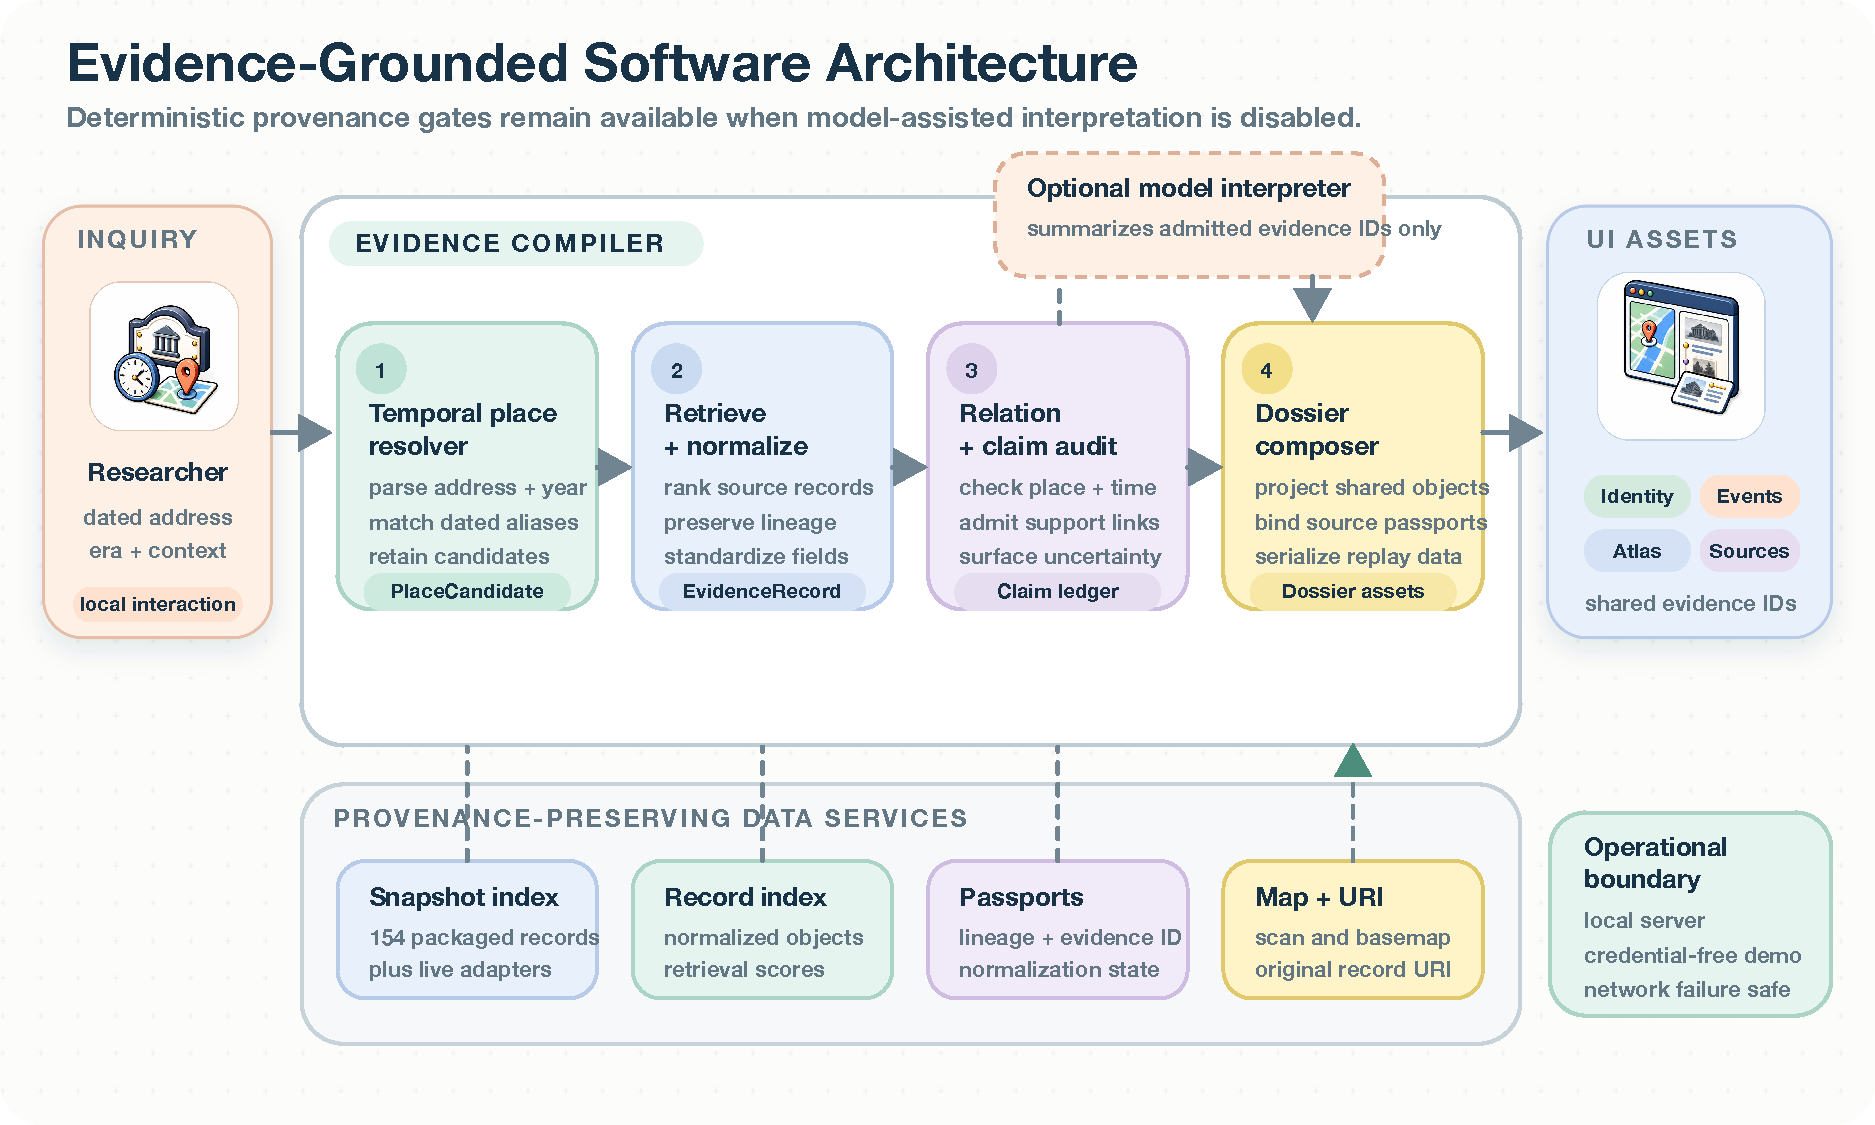
\includegraphics[width=0.94\textwidth]{assets/contextlens_architecture.pdf}
  \captionof{figure}{Software architecture. The deterministic evidence compiler mediates between a dated inquiry and four interface views. The optional model interpreter can summarize only evidence that has passed relation and claim gates. Dashed connections denote data-service or optional dependencies.}
  \label{fig:architecture}
\end{center}

\clearpage
\suppsection{Supplement B. Data Flow Pipeline}
\noindent
\begin{minipage}[t]{0.473\textwidth}
The pipeline distinguishes operations from the artifacts they produce (Figure~\ref{fig:dataflow}). Source records comprise the packaged official snapshot, catalog and map metadata, and open record URIs. Query Data contains the address string, temporal constraint, and optional contextual clue. Resolution and retrieval produce candidate place identities, ranked records, and the original source fields required for normalization.
\end{minipage}\hfill
\begin{minipage}[t]{0.473\textwidth}
Processing standardizes schemas, removes duplicates, and aligns temporal scopes. Its outputs are typed evidence objects, Source Passports, and linked entities. Analysis applies relation admission and claim auditing before optional model summarization. The renderer projects shared evidence objects into the Identity, Events, Atlas, and Sources views and the dossier JSON.
\end{minipage}
\vspace{10pt}

\begin{center}
  \centering
  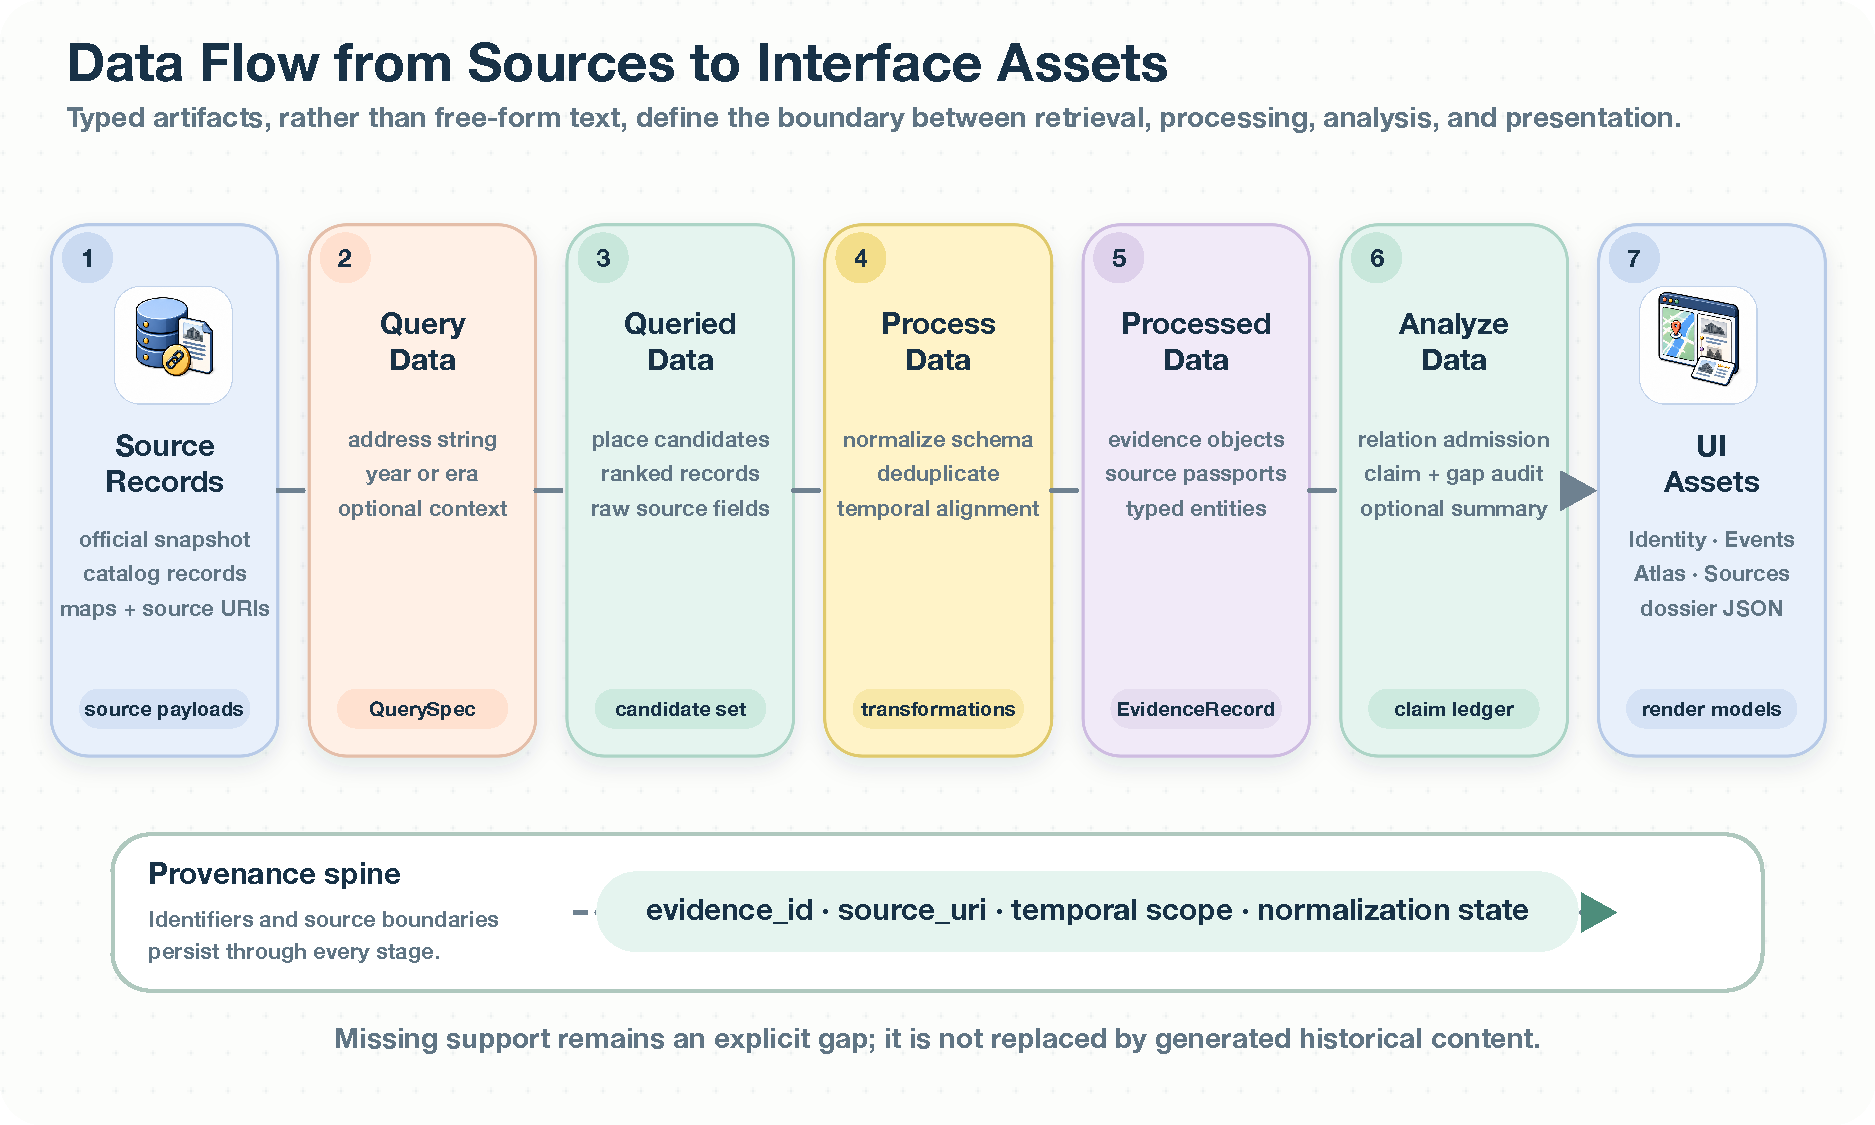
\includegraphics[width=0.94\textwidth]{assets/contextlens_data_flow.pdf}
  \captionof{figure}{Data flow from source records to interface assets. Each stage produces a named artifact, while the provenance spine preserves the evidence identifier, source URI, temporal scope, and normalization state across transformations.}
  \label{fig:dataflow}
\end{center}

\clearpage
\suppsection{Supplement C. Presentation Deliverable and Attribution}

\noindent
The ContextLens AAAI-27 presentation slide deck is a separate intellectual
deliverable from the demonstration paper, this technical supplement, the
software repository, the poster, and the demonstration video. The corresponding
author revised the deck's narrative structure, visual explanation of the
evidence compiler, distinction between ContextLens and StableTradeAtlas, and
presentation of team contributions. The deck incorporates system results and
figures produced by the project team, but its presentation narrative and visual
organization should not be treated as a formatting derivative of the paper.

\vspace{10pt}
\noindent
This attribution is recorded only in the appendix. It does not change the
authorship, technical claims, or evidence boundaries of the demonstration paper.

\vspace{14pt}
\noindent\textbf{Deliverable boundary.}
\vspace{4pt}

\renewcommand{\arraystretch}{1.22}
\noindent
\begin{tabularx}{\textwidth}{>{\raggedright\arraybackslash}p{0.16\textwidth}
  >{\raggedright\arraybackslash}p{0.36\textwidth}X}
\toprule
\textbf{Deliverable} & \textbf{Primary function} & \textbf{Relationship to the paper} \\
\midrule
Demo paper & Technical account of the system, demonstration scenario, and stated boundaries & Primary scholarly manuscript \\
Technical supplement & Software architecture, data flow, and this attribution record & Supporting appendix to the manuscript \\
Presentation slides & Conference presentation narrative and visual explanation & Separate intellectual deliverable revised by the corresponding author \\
Poster & One-page visual summary for browsing and discussion & Separate dissemination artifact \\
Software and video & Executable implementation and recorded interaction & Separate technical and media artifacts \\
\bottomrule
\end{tabularx}

\vspace{14pt}
\noindent\textbf{Archival record.}
The project repository preserves both the compiled slide deck and its editable
Beamer source. The source bundle includes \texttt{main.tex},
\texttt{references.bib}, and every figure required to reproduce the deck with
XeLaTeX. Keeping the source beside the browser-viewable PDF records the slide
deck as a revisable scholarly output rather than a static export.

\end{document}
